\documentclass{standalone}
\usepackage{tikz}
\usepackage{amsmath}
\usepackage[T1]{fontenc}
\tikzset{
    process/.style={draw, rectangle, rounded corners, fill=yellow!20, minimum width=1cm, auto, on grid, minimum height=1cm, align=center},
    process4/.style={draw, font=\fontsize{8}{9.6}\selectfont, rectangle, rounded corners, fill=yellow!20, text width=3cm, auto, on grid, align=center},
    decision/.style={draw, font=\fontsize{8}{9.6}\selectfont, rectangle, rounded corners, fill=red!20, text width=3cm, minimum height=1cm, auto, on grid, align=center},
    process2/.style={draw, font=\fontsize{8}{9.6}\selectfont, rectangle, rounded corners, fill=cyan!20, text width=4cm, auto, on grid, align=center},
    process3/.style={draw, font=\fontsize{8}{9.6}\selectfont, rectangle, text width=4cm, rounded corners, fill=cyan!20, rotate=-90, auto, on grid, align=center},
    vecArrow/.style={thick, decoration={markings,mark=at position 1 with {\arrow[semithick]{open triangle 60}}},
        double distance=1.4pt, shorten >= 5.5pt,
        preaction = {decorate},
        postaction = {draw,line width=1.4pt, white,shorten >= 4.5pt}},
    vecArrow1/.style={thick, decoration={markings,mark=at position 0.9 with {}},
        double distance=1.4pt, shorten >= 5.5pt,
        preaction = {decorate},
        postaction = {draw,line width=1.4pt, white,shorten >= 4.5pt}},
    innerWhite/.style={semithick, white,line width=1.4pt, shorten >= 4.5pt},
}

\usetikzlibrary{arrows, decorations.markings, arrows.meta,positioning,shadows,shapes.geometric,automata,positioning,fit,arrows.meta,calc,bending}


\usepackage{graphicx} % for including images

\usepackage{overpic} % for overlaying text on images

\begin{document}
\resizebox{0.7\textwidth}{!}{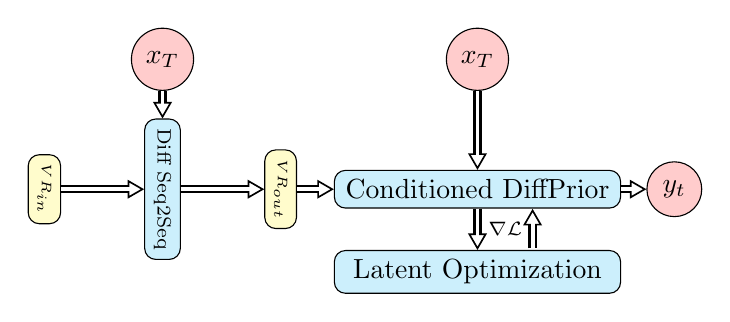
\begin{tikzpicture}[node distance=2cm]
\tikzstyle{process}=[draw, font=\fontsize{5}{4.8}\selectfont, rectangle, rounded corners, fill=yellow!20, minimum width=1cm, auto, on grid, minimum height=1cm, align=center]

\tikzstyle{decision}=[draw, font=\small, rectangle, rounded corners, fill=red!20, text width=3cm, auto, on grid, align=center]
\tikzstyle{process2}=[draw, font=\fontsize{9}{4.8}, rectangle, rounded corners, fill=cyan!20, text width=3.4cm, auto, on grid, align=center]
\tikzstyle{circlenode}=[draw, circle, fill=red!20, minimum size=1mm]
\tikzstyle{process3}=[draw, font=\fontsize{7}{4.8}\selectfont, rectangle, rounded corners, fill=cyan!20, rotate=-90, auto, on grid, align=center]
\tikzstyle{process4}=[draw, font=\fontsize{5}{4.8}\selectfont, rectangle, rounded corners, fill=yellow!20, rotate=-90, auto, on grid, align=center]
\tikzstyle{vecArrow} = [thick, decoration={markings, mark=at position 1 with {\arrow[semithick]{open triangle 60}}}, double distance=1.4pt, shorten >= 5.5pt, preaction = {decorate}, postaction = {draw, line width=1.4pt, white, shorten >= 4.5pt}]
\tikzstyle{vecArrow1} = [thick, decoration={markings, mark=at position 0.9 with {}}, double distance=1.4pt, shorten >= 5.5pt, preaction = {decorate}, postaction = {draw, line width=1.4pt, white, shorten >= 4.5pt}]
\tikzstyle{innerWhite} = [semithick, white, line width=1.4pt, shorten >= 4.5pt]

\node[process4] (input) at (-4.5, -0.35) {${VR}_{in}$};
\node[process3] (seq2seq) at (-3, -0.35) {Diff Seq2Seq};
\draw[vecArrow] (input) -- (seq2seq);
\node[process4] (output) at (-1.5, -0.35) {${VR}_{out}$};
\draw[vecArrow] (seq2seq) -- (output);
\node[process2] (prior) at (1, -0.35) {Conditioned DiffPrior};
\node[circlenode] (yt) at (3.5, -0.35){$y_t$};
\node[circlenode] (xt) at (1, 1.3){$x_T$};
\node[circlenode] (xt1) at (-3, 1.3){$x_T$};
\draw[vecArrow] (prior) -- (yt);
\draw[vecArrow] (xt1) -- (seq2seq);
\draw[vecArrow] (xt) -- (prior);

\draw[vecArrow] (output) -- (prior);
\node[process2] (optimization) at (1, -1.4) {Latent Optimization};
\draw[vecArrow] (prior) -- (optimization);
\draw[vecArrow] (1.7, -1.1) tonode[anchor=east] {\scriptsize $\nabla \mathcal{L}$} (1.7, -0.6);


\end{tikzpicture}}
\end{document}